%%%%%%%%%%%%%%%%%%%%%%%%%%%%%%%%%%%%%%%%%
% baposter Landscape Poster
% LaTeX Template
% Version 1.0 (11/06/13)
%
% baposter Class Created by:
% Brian Amberg (baposter@brian-amberg.de)
%
% This template has been downloaded from:
% http://www.LaTeXTemplates.com
%
% License:
% CC BY-NC-SA 3.0 (http://creativecommons.org/licenses/by-nc-sa/3.0/)
%
%%%%%%%%%%%%%%%%%%%%%%%%%%%%%%%%%%%%%%%%%

%----------------------------------------------------------------------------------------
%	PACKAGES AND OTHER DOCUMENT CONFIGURATIONS
%----------------------------------------------------------------------------------------

\documentclass[landscape,a0paper,fontscale=0.285]{baposter} % Adjust the font scale/size here

\usepackage{graphicx} % Required for including images
\graphicspath{{figures/}} % Directory in which figures are stored

\usepackage{amsmath} % For typesetting math
\usepackage{amssymb} % Adds new symbols to be used in math mode

\usepackage{booktabs} % Top and bottom rules for tables
\usepackage{enumitem} % Used to reduce itemize/enumerate spacing
\usepackage{palatino} % Use the Palatino font
\usepackage[font=small,labelfont=bf]{caption} % Required for specifying captions to tables and figures

\usepackage{multicol} % Required for multiple columns
\setlength{\columnsep}{1.5em} % Slightly increase the space between columns
\setlength{\columnseprule}{0mm} % No horizontal rule between columns

\usepackage{tikz} % Required for flow chart
\usetikzlibrary{shapes,arrows} % Tikz libraries required for the flow chart in the template

\newcommand{\compresslist}{ % Define a command to reduce spacing within itemize/enumerate environments, this is used right after \begin{itemize} or \begin{enumerate}
\setlength{\itemsep}{1pt}
\setlength{\parskip}{0pt}
\setlength{\parsep}{0pt}
}

\definecolor{lightblue}{rgb}{0.145,0.6666,1} % Defines the color used for content box headers

\begin{document}

\begin{poster}
{
headerborder=closed, % Adds a border around the header of content boxes
colspacing=1em, % Column spacing
bgColorOne=white, % Background color for the gradient on the left side of the poster
bgColorTwo=white, % Background color for the gradient on the right side of the poster
borderColor=lightblue, % Border color
headerColorOne=black, % Background color for the header in the content boxes (left side)
headerColorTwo=lightblue, % Background color for the header in the content boxes (right side)
headerFontColor=white, % Text color for the header text in the content boxes
boxColorOne=white, % Background color of the content boxes
textborder=roundedleft, % Format of the border around content boxes, can be: none, bars, coils, triangles, rectangle, rounded, roundedsmall, roundedright or faded
eyecatcher=true, % Set to false for ignoring the left logo in the title and move the title left
headerheight=0.1\textheight, % Height of the header
headershape=roundedright, % Specify the rounded corner in the content box headers, can be: rectangle, small-rounded, roundedright, roundedleft or rounded
headerfont=\Large\bf\textsc, % Large, bold and sans serif font in the headers of content boxes
%textfont={\setlength{\parindent}{1.5em}}, % Uncomment for paragraph indentation
linewidth=2pt % Width of the border lines around content boxes
}
%----------------------------------------------------------------------------------------
%	TITLE SECTION 
%----------------------------------------------------------------------------------------
%
{
\includegraphics[height=4em]{logo.png}} % First university/lab logo on the left
{\bf\textsc{Drone Mounted Sensor Networks}\vspace{0.5em}} % Poster title
{\textsc{\{ Alex Henson, Ben De Ivey, Jon Gibson, and William Seymour \} \hspace{12pt} Computer Science, University of Warwick}} % Author names and institution
{
\includegraphics[height=4em]{logo.png}} % Second university/lab logo on the right

%----------------------------------------------------------------------------------------
%	OBJECTIVES
%----------------------------------------------------------------------------------------

\headerbox{Objectives}{name=objectives,column=1,row=0}{

This project focuses on methods by which such networks can be controlled and tasked. We are working to create a framework by which autonomous flying vehicles can be tasked remotely to map sensor properties over predefined areas. This encompasses:

\begin{enumerate}\compresslist
\item Routing of drones through shared airspace
\item Routing of communications
\item Specification of tasking language
\item Fault tolerance of the network
\item Division and dissemination of instructions
\end{enumerate}
}

%----------------------------------------------------------------------------------------
%	INTRODUCTION
%----------------------------------------------------------------------------------------

\headerbox{Introduction}{name=introduction,column=0,row=0,bottomaligned=objectives}{

A great amount of work has gone into research surrounding sensor networks in recent years, and the explosion in popularity of the internet of things (IoT) means there is a great deal of support from both academia and industry for development in the field. 

The use of quadcopters (and drones in general) has also increased in both the civilian and military sectors. By combining the power of distributed sensor networks with the manoeuvrability of unmanned drones it is possible to quickly survey and map properties over a large area.
}
%----------------------------------------------------------------------------------------
%	RESULTS 1
%----------------------------------------------------------------------------------------

\headerbox{Communications Routing}{name=results,column=2,span=2,row=0}{

\begin{multicols}{2}
\vspace{1em}

Mobile Ad-hoc Networks (MANETs) have several distinguishing characteristics which must be accounted for when designing and evaluating routing algorithms\cite{macker1999mobile}:

\begin{enumerate}\compresslist
\item Dynamic topologies
\item Bandwidth-constrained, variable capacity links
\item Energy-constrained operation
\item Limited physical security
\end{enumerate}

All electromagnetic signals dissipate as they propagate through space, limiting the range at which communications can be received. Under ideal conditions this can be modelled using the Friis free space equation:

\begin{equation}
P_{rx} = P_{tx}G_{tx}G_{rx}\frac{\lambda^2}{4{\pi}D}
\label{friis}
\end{equation} 

Where $P$ is the power of the radio signal, $G$ the gain (or efficiency) of the antenna and $D$ the distance between them. Under real world conditions additional path loss can be modelled  using the log distance path loss model:

\begin{equation}
L = 10n {\log_{10}}d + C
\end{equation}

Multiple algorithms exist to route packets within a network, which are usually classified into topological and positional. For mobile networks, topological models are ineffective due to the aforementioned dynamic topologies employed.
\newline

Ad hoc On-Demand Distance Vector (AODV) routing is one of the most popular reactive protocols used in MANETS\cite{perkins2003ad}. When a node wishes to send a message but does not have a route to the destination, it broadcasts a route request (RREQ) packet to it's neighbours. Each neighbour either returns a route if it has one (RREP) or rebroadcasts the RREQ to it's own neighbours. Sequence numbers are used to eliminate suboptimal routes and by extension to prevent cyclical routes.

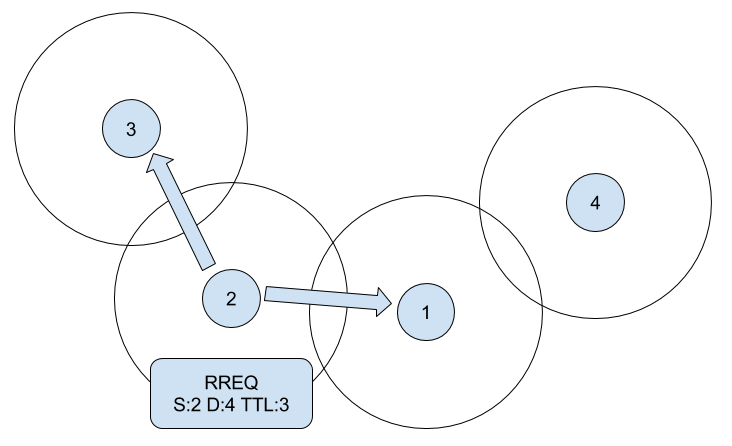
\includegraphics[scale=0.25]{figures/aodv-1}

If the network topology has changed and a route is invalid, a node returns a route error (RERR) message. This causes other nodes to flush the parts of their routing tables which have become invalid. AODV does not have a security component, but this can be added separately. As all nodes in the network are known beforehand, keys can be distributed prior to deployment.
\newline

For MANETS, reactive protocols like AODV are preferred to proactive protocols (such as OLSR) due to low power and processing requirements.
\end{multicols}
}

%----------------------------------------------------------------------------------------
%	REFERENCES
%----------------------------------------------------------------------------------------

\headerbox{Project Management}{name=references,column=0,above=bottom}{
Integer sed lectus vel mauris euismod suscipit. Praesent a est a est ultricies pellentesque. Donec tincidunt, nunc in feugiat varius, lectus lectus auctor lorem, egestas molestie risus erat ut nibh.
}

%----------------------------------------------------------------------------------------
%	FUTURE RESEARCH
%----------------------------------------------------------------------------------------

\headerbox{References}{name=futureresearch,column=1,span=3,aligned=references,above=bottom}{ % This block is as tall as the references block

\begin{multicols}{3}
\renewcommand{\section}[2]{\vskip 0.05em} % Get rid of the default "References" section title
\nocite{*} % Insert publications even if they are not cited in the poster
\footnotesize{ % Reduce the font size in this block
\bibliographystyle{unsrt}
\bibliography{bibliography} % Use sample.bib as the bibliography file
}
\end{multicols}
}

%----------------------------------------------------------------------------------------
%	CONTACT INFORMATION
%----------------------------------------------------------------------------------------

%\headerbox{Respository}{name=contact,column=3,aligned=references,above=bottom}{ % This block is as tall as the references block

%\begin{description}\compresslist
%\item[Web] https://github.com/mcnutty26/effacious-octo-weasel
%\end{description}
%}

%----------------------------------------------------------------------------------------
%	CONCLUSION
%----------------------------------------------------------------------------------------

\headerbox{Planned Work}{name=conclusion,column=2,span=2,row=0,below=results,above=references}{

\begin{multicols}{2}

\begin{itemize}\compresslist
\item Pellentesque eget orci eros. Fusce ultricies, tellus et pellentesque fringilla, ante massa luctus libero, quis tristique purus urna nec nibh. Phasellus fermentum rutrum elementum. Nam quis justo lectus.
\item Vestibulum sem ante, hendrerit a gravida ac, blandit quis magna.
\item Donec sem metus, facilisis at condimentum eget, vehicula ut massa. Morbi consequat, diam sed convallis tincidunt, arcu nunc.
\item Nunc at convallis urna. isus ante. Pellentesque condimentum dui. Etiam sagittis purus non tellus tempor volutpat. Donec et dui non massa tristique adipiscing.
\end{itemize}

\end{multicols}
}

%----------------------------------------------------------------------------------------
%	MATERIALS AND METHODS
%----------------------------------------------------------------------------------------

\headerbox{Simulation Tools}{name=method,column=0,below=objectives,bottomaligned=conclusion}{ % This block's bottom aligns with the bottom of the conclusion block

The following materials were required to complete the research:

\begin{itemize}\compresslist
\item Curabitur pellentesque dignissim
\item Eu facilisis est tempus quis
\item Duis porta consequat lorem
\item Eu facilisis est tempus quis
\end{itemize}

The following equations were used for statistical analysis:

\begin{equation}
\cos^3 \theta =\frac{1}{4}\cos\theta+\frac{3}{4}\cos 3\theta
\label{eq:refname}
\end{equation}\

\begin{equation}
E = mc^{2}
\label{eqn:Einstein}
\end{equation}

Phasellus imperdiet, tortor vitae congue bibendum, felis enim sagittis lorem, et volutpat ante orci sagittis mi. Morbi rutrum laoreet semper. Morbi accumsan enim nec tortor consectetur non commodo nisi sollicitudin. Proin sollicitudin. Pellentesque eget orci eros. Fusce ultricies, tellus et pellentesque fringilla, ante massa luctus libero, quis tristique purus urna nec nibh.
}

%----------------------------------------------------------------------------------------
%	RESULTS 2
%----------------------------------------------------------------------------------------

\headerbox{Physical Routing}{name=results2,column=1,below=objectives,bottomaligned=conclusion}{ % This block's bottom aligns with the bottom of the conclusion block

Donec faucibus purus at tortor egestas eu fermentum dolor facilisis. Maecenas tempor dui eu neque fringilla rutrum. Mauris \emph{lobortis} nisl accumsan.

\begin{center}
\begin{tabular}{l l l}
\toprule
\textbf{Treatments} & \textbf{Response 1} & \textbf{Response 2}\\
\midrule
Treatment 1 & 0.0003262 & 0.562 \\
Treatment 2 & 0.0015681 & 0.910 \\
Treatment 3 & 0.0009271 & 0.296 \\
\bottomrule
\end{tabular}
\captionof{table}{Table caption}
\end{center}

Nulla ut porttitor enim. Suspendisse venenatis dui eget eros gravida tempor. Mauris feugiat elit et augue placerat ultrices. Morbi accumsan enim nec tortor consectetur non commodo.

\begin{center}
\begin{tabular}{l l l}
\toprule
\textbf{Treatments} & \textbf{Response 1} & \textbf{Response 2}\\
\midrule
Treatment 1 & 0.0003262 & 0.562 \\
Treatment 2 & 0.0015681 & 0.910 \\
Treatment 3 & 0.0009271 & 0.296 \\
\bottomrule
\end{tabular}
\captionof{table}{Table caption}
\end{center}
}

%----------------------------------------------------------------------------------------

\end{poster}

\end{document}